%% This is file 'chapter1.tex'
%% It is included by hhuthesis-example.tex for hhuthesis.
%%
%% Copyright(C) 2020-2021, Wenhan Cao
%% College of Water Conservancy and Hydropower Engineering, Hohai University.
%%
%% Version:v2.0.0
%% Last update: April 7th, 2021.
%%
%% Home Page of the Project: https://github.com/caowenhan/thesis
%%
%% This file may be distributed and / or modified under the conditions of the
%% LaTeX Project Public License, either version 1.3c of this license or (at your
%% option) any later version. The latest version of this license is in:
%%
%% http://www.latex-project.org/lppl.txt
%%
%% and version 1.3c or later is part of all distributions of LaTeX version
%% 2008/05/04 or later.
%%
\chapter{引言}
\label{chap:introduction}
\section{MeV 伽马天文物理背景}
\label{sec:meaning}

作为高能天体物理研究的重要窗口,MeV伽马射线天文学正成为探索极端宇宙的新前沿。在伽马射线能谱中,0.1--100 MeV能段承载着独特的物理信息:该能域覆盖了正负电子湮灭线(511 keV),
放射性元素衰变线(如 $^{26}$Al 的 1.809 MeV 线)、脉冲星曲率辐射峰值等特征辐射,同时也是研究暗物质粒子湮灭/衰变信号、原初黑洞蒸发效应的关键探测窗口。然而受制于康普顿望远镜的空间
分辨限制和探测效率瓶颈,该能段的系统观测长期处于“MeV 能量间隙”的状态,这也使得MeV伽马天空仍存在大量未解之谜。因此,开发高能分辨率、大视场、高探测效率的MeV伽马望远镜成为
高能天文学界的共同迫切需求。\par
当前学界内围绕该能段已形成若干突破方向:在观测技术层面,康普顿成像与电子追踪技术的结合正在实现MeV偏振测量,这将为揭示伽马暴中心引擎结构、耀变体喷流磁流体特性提供新维度;
在理论建模方面,MeV耀变体的特殊光变特征挑战着传统轻子模型,推动着强子主导辐射机制和粒子加速过程的研究;而通过MeV谱线巡天发现的银河系暗物质晕湮灭信号,正与Sub-GeV能段的
原初黑洞蒸发伽马射线形成交叉验证,为解开暗物质本质之谜开辟新路径。这些研究方向共同构成了连接微观粒子物理与宏观宇宙演化的关键纽带,正在重塑我们对极端天体环境、早期宇宙遗迹
和基本物理规律的理解框架。\par
\subsection{$\pi$介子鼓包}
\label{subsec:pion}
在MeV伽马射线天文学的研究框架下,超新星遗迹作为银河系宇宙线加速源的核心地位正经历革命性观测验证。理论模型指出,这类遗迹的激波波前通过扩散激波加速(DSA)机制,可将质子加速至PeV能级
(即"膝区"能量),其过程中高能质子与星际介质碰撞产生的中性$\pi^{0}$介子衰变($\pi^{0} \rightarrow 2\gamma$),会在$\gamma$射线能谱的50-200 MeV区间形成特征性鼓包结构——这被视为宇宙线
强子加速过程的"指纹证据"。然而,现有伽马望远镜在MeV能段的灵敏度缺失,导致该关键谱形长期无法被完整解析:Fermi-LAT在GeV以上能区虽已观测到多个遗迹的强子辐射成分(如IC 443和W44中2.2 MeV中子俘获线的关联信号),
但无法区分10-300 MeV能段内轻子同步辐射与强子$\pi^{0}$衰变的混合贡献;而COMPTEL等早期MeV探测器受限于>3°的角分辨率,难以实现致密遗迹的空间分辨谱诊断。
\begin{figure}[H]
	\centering
	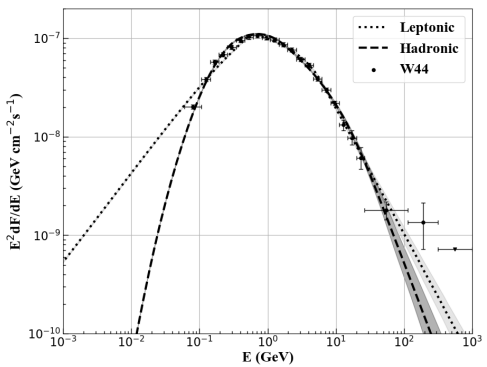
\includegraphics[width=0.7\textwidth]{figures/Pi介子鼓包.png}
	\caption{$\pi$介子鼓包} \label{fig:pion}
	%硕士论文、本科毕业论文不使用双语图表标题,可使用命令\caption{}替代\caption{}
\end{figure}
\subsection{暗物质与原初黑洞}
\label{subsec:darkmatter}
在暗物质本质的百年探寻中,原初黑洞(Primordial Black Holes, PBHs)因其诞生于宇宙早期相变的独特属性,始终占据着候选者名单的核心位置。根据霍金辐射理论,质量在$10^{16}-10^{17}g$范围内的PBHs
正处于蒸发末期,其事件视界量子隧穿效应会释放以光子为主导的粒子流,形成特征性的keV-MeV能段热辐射谱——这一能域恰与MeV伽马天文观测的核心敏感区间高度契合。理论计算表明,单个蒸发PBH的瞬时伽马辐射流量在1 MeV处可达
$10^{-7}MeV/(cm^2s)$量级。,其全天空累积辐射更可能构成弥漫性MeV背景辐射的未解析成分。这使得MeV能段成为检验PBH暗物质假说的"战略频段":通过精确测量宇宙伽马背景能谱的软X射线至MeV能段(0.1-10 MeV)的谱形畸变,
可直接约束PBH质量分布函数$f_{PBH}(M)$在关键参数空间($M \sim 10^{16} g$)的分布,进而验证或排除PBH作为暗物质的可能性。
然而,这一科学目标的实现长期受困于两大技术壁垒:其一,蒸发PBH的辐射信号在MeV能段呈现宽谱特性($dN/dE \propto E_{-3} $),易与活动星系核(AGN)的幂律辐射、超新星遗迹的π⁰衰变连续谱等天体物理背景混淆;
其二,现有康普顿望远镜(如COMPTEL)在1 MeV附近的灵敏度仅达$10^{-5} MeV/(cm^2 s)$,难以探测PBH蒸发预期的微弱各向异性信号。
\begin{figure}[H]
	\centering
	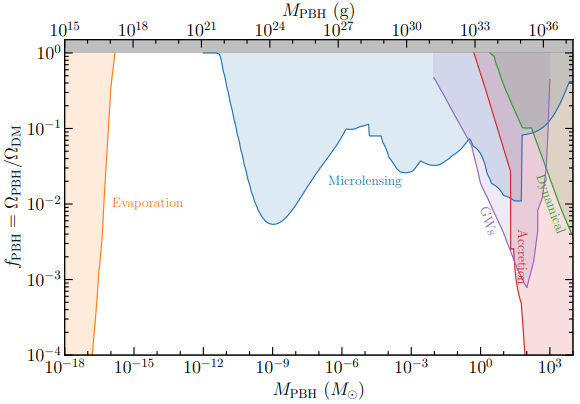
\includegraphics[width=0.7\textwidth]{figures/暗物质与原初黑洞.png}
	\caption{暗物质与原初黑洞} \label{fig:darkmatter}
	%硕士论文、本科毕业论文不使用双语图表标题,可使用命令\caption{}替代\caption{}
\end{figure}

\section{装置指标需求}

\subsection{科学目标}
在MeV伽马射线天文学领域,该能段(0.1-100 MeV)因其独特的物理信息承载能力,成为探索极端宇宙现象的战略窗口。其科学目标涵盖多个前沿方向:
\subsubsection{宇宙线起源与超新星遗迹研究}
	超新星遗迹激波加速的高能质子与星际介质碰撞产生中性π⁰介子衰变,其辐射在50-200 MeV能段形成特征鼓包谱。现有设备如Fermi-LAT在GeV以上能区观测到强子成分,
	但MeV能段的混合辐射(轻子同步与强子π⁰衰变)需角分辨率优于1°以实现空间分辨谱诊断,例如MeGaT望远镜通过三维径迹重建将角分辨率提升至0.8°@100 MeV,
	显著提高了谱形畸变检测能力。
\subsubsection{暗物质与原初黑洞探测}
	质量在$10^{16}-10^{17}g$范围内的原初黑洞PBHs,通过霍金辐射释放keV-MeV能段的光子,其累积辐射可能构成未解析的弥漫性背景。
	通过MeV能谱畸变分析,可约束PBH质量分布函数$f_{PBH}(M)$,但需灵敏度达$10^{-8}MeV/(cm^2s)$的高能分辨率望远镜量级以区分天体物理背景(如活动星系核的幂律辐射)。
	此外,暗物质粒子湮灭(如WIMP模型)可能产生511 keV正负电子湮灭线或宽谱信号,需亚度级角分辨率以定位银河系暗物质晕的空间分布。
\subsubsection{高能天体物理过程与多信使天文学}
	高能天体物理过程(如脉冲星曲率辐射、伽马暴中心引擎结构)的研究,对MeV能段的高能分辨率、大视场、高探测效率望远镜提出了挑战。
	伽玛射线暴(GRB)中心引擎的黑洞超吸积系统(NDAF)释放的MeV中微子与伽马射线存在关联,需时间投影室(TPC)与像素化碲锌镉(CZT)探测器的复合结构实现符合测量,
	以抑制本底并捕捉亚毫秒级爆发信号。此外,耀变体喷流的磁流体特性研究依赖MeV偏振测量,要求偏振度探测精度达5\%以内。
\subsection{对探测装置的核心指标需求}

\subsubsection{灵敏度突破}
	MeGaT望远镜的核心指标需求之一是在MeV能段实现灵敏度突破,以探测超新星遗迹的π⁰介子鼓包、暗物质原初黑洞的蒸发辐射等关键信号。在MeV能段,MeGaT望远镜的灵敏度需达到$10^{-8}MeV/(cm^2s)$量级,较传统康普顿望远镜(如COMPTEL)优化2-3个量级,以捕捉PBH蒸发和暗物质湮灭的微弱信号。	
\subsubsection{角分辨率提升}
	MeGaT望远镜的核心指标需求之二是在MeV能段实现角分辨率提升,以区分超新星遗迹的强子π⁰衰变与轻子同步辐射的混合贡献。在100 MeV处,MeGaT望远镜的角分辨率需达到0.8°,通过TPC的三维径迹重建与CZT的高位置分辨率,实现亚度级定位(如0.8°@100 MeV),从而区分密集天体源并解析π⁰鼓包谱形。
\subsubsection{偏振度探测}
	MeGaT望远镜的核心指标需求之三是在MeV能段实现偏振度探测,以研究耀变体喷流的磁流体特性。MeGaT望远镜的偏振度探测精度需达到5\%以内,以实现高精度的偏振测量。
\subsubsection{本底抑制技术}
	MeGaT望远镜的核心指标需求之四是在MeV能段实现偏本底抑制。
	采用双探测模态(如TPC+CZT)的符合测量,结合时间-能量-空间多维筛选,使本底抑制效率达$10^{4}$量级,例如通过抗辐照SiPM技术降低噪声干扰。
\subsubsection{空间分辨率}
	MeGaT望远镜的核心指标需求之五是在MeV能段实现空间分辨率,以定位银河系暗物质晕的空间分布。MeGaT望远镜的空间分辨率需达到亚度级,以实现高精度的空间分布测量。
	
\section{MeV伽马射线望远镜的国内外研究现状}
\label{sec:status}
MeV伽马射线天文学是高能天体物理研究的重要分支,其研究对象包括超新星遗迹、暗物质、原初黑洞等。MeV伽马射线天文学的研究方法主要包括观测、理论模拟和数据分析等。目前,国际上已经有多个MeV伽马射线望远镜项目,如Fermi-LAT、COMPTEL等,
这些望远镜在MeV能段的观测数据为MeV伽马射线天文学的研究提供了重要的信息。\par
此外,国际上还有一些关于MeV伽马射线天文学的理论模拟和数据分析的研究工作,这些工作为MeV伽马射线天文学的研究提供了理论基础和数据支持。\par
\subsection{HARPO:伽马射线偏振测量与角度测量}
\subsubsection{HARPO的科学目标}

\subsubsection{HARPO的工作原理}

\subsubsection{HARPO的实验配置}
	HARPO原型是一个30厘米立方体的TPC,可以在低压力至5巴的压力下操作。它被6个闪烁体板包围,提供外部触发信号。放大过程由两个GEM(气体电子倍增器)和一个
	micromegas组成。读出系统包括两个系列(x, y, 垂直于彼此)的288个铜条,间距为1毫米。

	\begin{figure}[htbp]
		\centering
		\begin{subfigure}[b]{0.45\textwidth}
			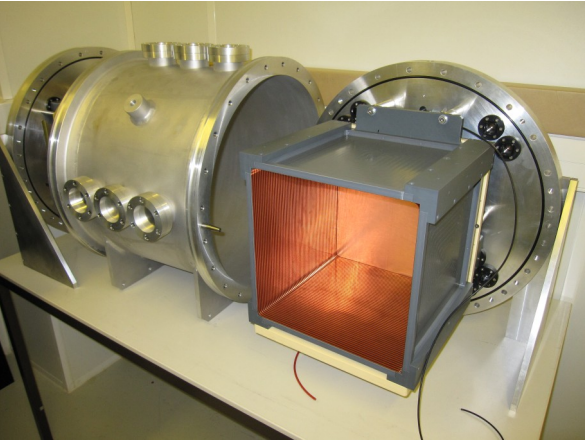
\includegraphics[width=0.75\textwidth]{figures/HA演示装置.png}
			\caption{HA演示装置}
			\label{fig:sub1}
		\end{subfigure}
		\hspace{0.01\textwidth} % 调整间距
		\begin{subfigure}[b]{0.45\textwidth}
			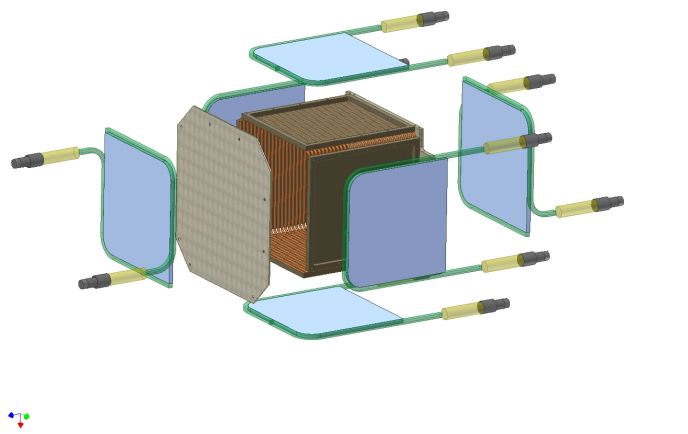
\includegraphics[width=0.75\textwidth]{figures/HA设计草图.png}
			\caption{HA设计草图}
			\label{fig:sub2}
		\end{subfigure}
		\caption{HARPO的实验配置}
		\label{fig:figures}
	\end{figure}
\subsubsection{HARPO的实验模拟}
HARPO 探测器的立方设计使得其解析解不可得,文章中采用数值模拟的方法去模拟探测器的响应。它包括:\par
• 提供正负电子对能量动量的光子转换事件发生器;\par
• 基于 Geant4,模拟正负电子对与气体的相互作用;\par
• 对 TPC 工作过程和几何形状的描述的模块,它提供了与真实数据类似的信号图。
\begin{figure}[H] %H为当前位置,!htb为忽略美学标准,htbp为浮动图形
	\centering %图片居中
	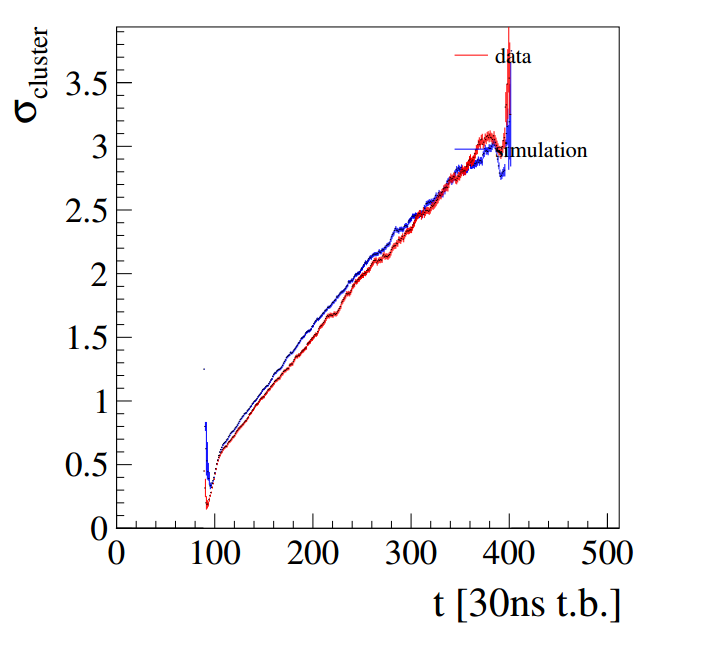
\includegraphics[width=0.55\textwidth]{Figures/校正漂移信号结果.png} %插入图片,[]中设置图片大小,{}中是图片文件名
	\caption{数据(红色)和模拟(蓝色)中宇宙射线样本的信号大小(有效值)与漂移距离的函数关系,可见数据和模拟结果非常吻合} %最终文档中希望显示的图片标题
\end{figure}
\subsubsection{HARPO的数据分析}
1.偏振测量结果\par
使用HARPO开发的一个特定的重建算法来重建TPC中的顶点,从而提取电子和正电子的方位角$\phi_{+-}$。$\phi_{+-}$的分布预期将遵循一个包含偏振不对称性A和偏振方向$\phi_{0}$的分布。
通过将极化和非极化光子的$\phi_{+-}$分布相除,可以消除系统误差。结果如图:
\begin{figure}[H] %H为当前位置,!htb为忽略美学标准,htbp为浮动图形
	\centering %图片居中
	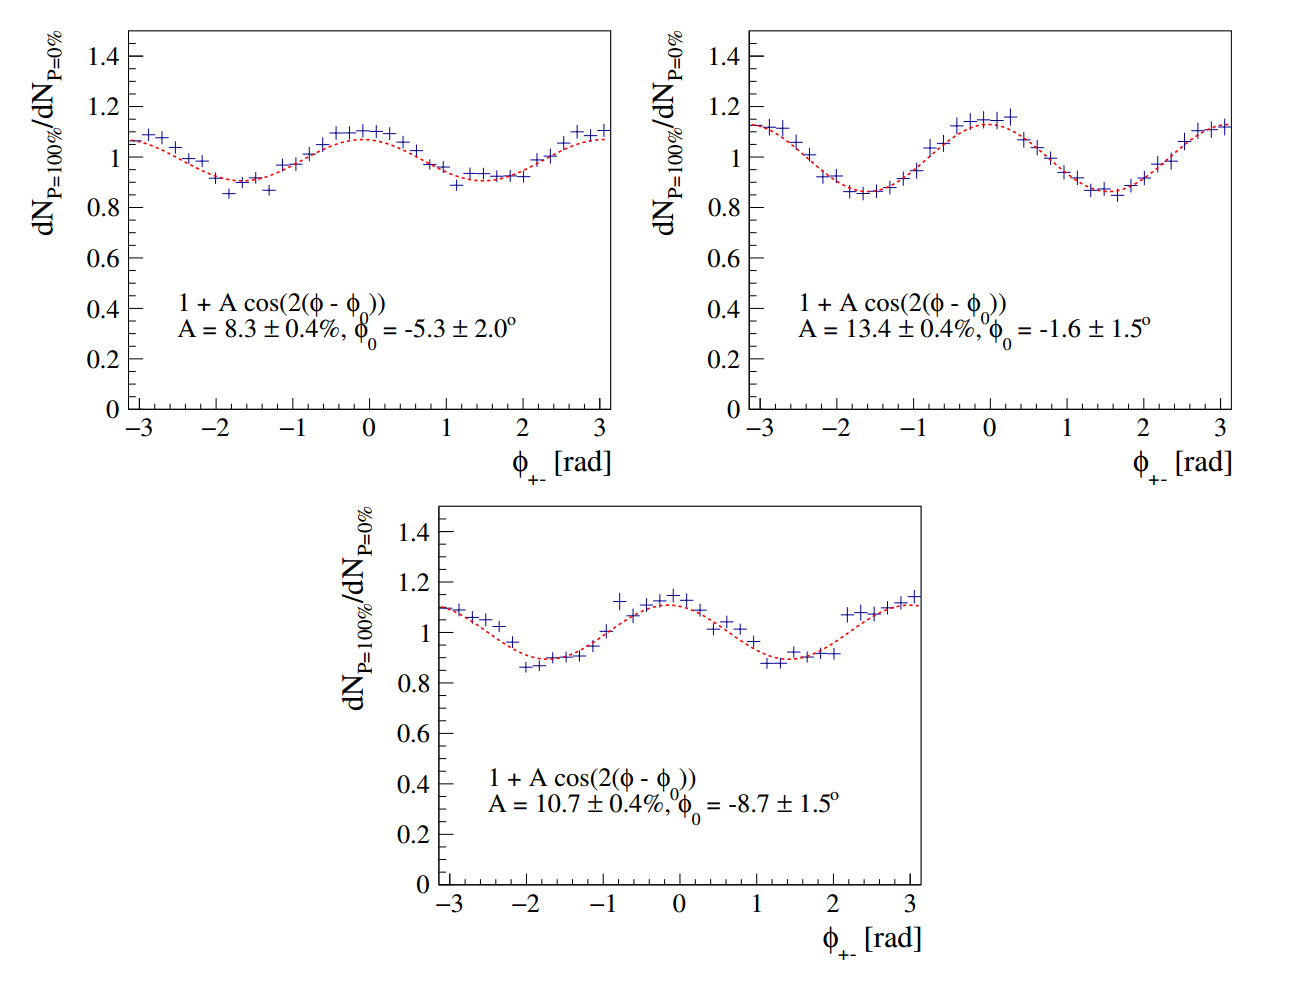
\includegraphics[width=0.7\textwidth]{figures/18HA测量结果.png} %插入图片,[]中设置图片大小,{}中是图片文件名
	\caption{11.8 MeV 光子束的极化调制(左上角两个分布均为真实数据。右上角两种分布都是模拟的。下图中偏振光分布来自真实光束数据,非偏振光分布来自模拟数据)} %最终文档中希望显示的图片标题
\end{figure}
2.角度测量结果\par
• 未能直接测量反冲核的动量大小,其贡献记作$\sigma_{recoil}$;\par
• 未能直接测量两个粒子的动量大小,其贡献记为$\sigma_{p}$;\par
• 对单个带电粒子探测器视域(场)有限。
将$\sigma_{\theta,68\%}$记作粒子数68\%的包含角(即距$\sigma_{\theta}$平均值一个标准差内),模拟部分结果如图:
\begin{figure}[htbp]
	\centering
	\begin{subfigure}[b]{0.45\textwidth}
		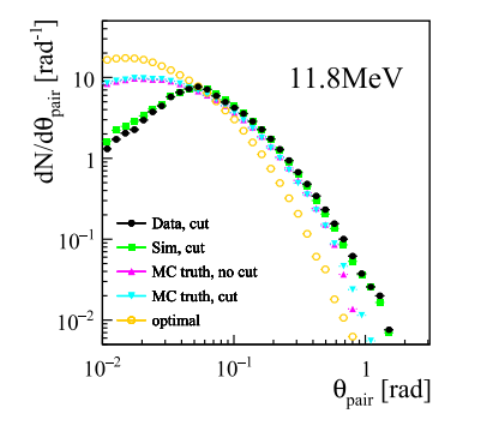
\includegraphics[width=0.75\textwidth]{figures/探测器模拟结果.png}
		\caption{11.8 MeV 光子光束的残角$\theta$对分布。黑点为光束测量值。黄色圆圈显示的是使用了蒙特卡洛的全部4向量信息的QED极限。
		洋红色三角形显示的是仅使用蒙特卡洛中的轨道方向(动量大小未知)得出的残差,青色三角形显示的是开角剪切对该分布的影响。
		绿色正方形显示的是考虑了整个探测器模拟的分布,包括康普顿和三重事件的污染。数据与全探测器模拟一致。}
		\label{fig:sub3}
	\end{subfigure}
	\hspace{0.01\textwidth} % 调整间距
	\begin{subfigure}[b]{0.45\textwidth}
		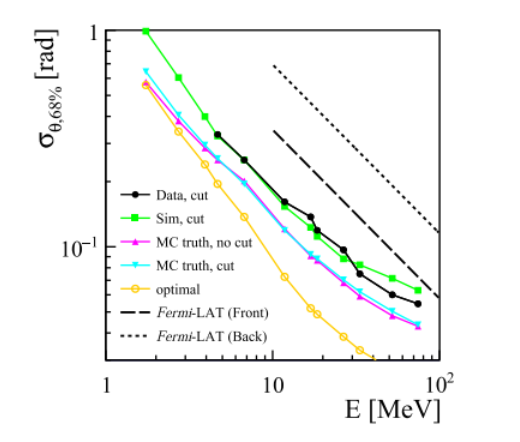
\includegraphics[width=0.75\textwidth]{figures/角分辨率与能量关系.png}
		\caption{68\%包容角与光束能量的函数关系。黑点表示在光束中的测量结果。绿色正方形显示的是模拟的结果,
		包括康普顿和三重事件的污染。洋红色三角形只考虑在没有动量大小测量的情况下的QED极限。
		青色三角形只考虑事件选择对分辨率的影响。黄色圆圈表示在不测量反冲核的情况下的QED极限。
		虚线和点线表示费米-LAT对前转换和后转换事件的角度分辨率。}
		\label{fig:sub4}
	\end{subfigure}
	\caption{HARPO的实验模拟结果}
	\label{fig:figures2}
\end{figure}


\subsection{e-ASTROGAM: 伽马射线天文学的新视野}

\subsubsection{e-ASTROGAM的科学动机}

\subsubsection{e-ASTROGAM的设计目标}

\subsubsection{e-ASTROGAM的仪器设计}

\subsubsection{e-ASTROGAM的仪器优势}

\subsubsection{e-ASTROGAM的数据分析}



\subsection{MeGaT望远镜的研究前景}
MeGaT望远镜是一种新型的MeV伽马射线望远镜,具有高能分辨率、大视场、高探测效率等优点。MeGaT望远镜的研究前景非常广阔,可以应用于超新星遗迹、暗物质、原初黑洞等领域的研究。未来,MeGaT望远镜有望成为MeV伽马射线天文学研究的重要工具,为我们揭示宇宙的奥秘提供重要的信息。\par


\section{MeGaT 实验方案与指标预期}
\label{sec:plan}
\subsection{MeGaT实验方案}
MeGaT(MeV Gamma-ray Telescope)探测系统作为新一代高气压时间投影室(TPC)技术的里程碑式应用,其创新性架构旨在突破MeV伽马天文长期面临的空间分辨与灵敏度瓶颈。该系统采用双模态复合探测器设计,
通过高气压TPC+Micromegas电子径迹成像模块与像素化半导体/闪烁体量能器的协同工作,实现了对康普顿散射过程的全事件重建:
\subsubsection{TPC+Micromegas电子径迹重建模块}
	TPC+Micromegas电子径迹重建模块是MeGaT探测系统的核心部件,其主要功能是实现高能分辨率、大视场、高探测效率的MeV伽马射线探测。该模块采用高气压TPC技术,结合Micromegas电子径迹成像技术,
	实现了对MeV伽马射线的高能分辨率探测。该模块的设计和制造工艺对MeGaT探测系统的性能有重要影响,是MeGaT探测系统的关键技术之一。
	基于10 bar氙基气体环境,康普顿散射电子在TPC内产生电离径迹,通过Micromegas微网探测器实现三维径迹重建,空间分辨率达0.3 mm(RMS),角分辨率达0.8°@100 MeV。\par
\subsubsection{像素化半导体/闪烁体量能器}
	像素化半导体/闪烁体量能器是MeGaT探测系统的辅助部件,其主要功能是实现对MeV伽马射线的高能量分辨率探测。该模块采用像素化半导体/闪烁体量能器技术,结合TPC+Micromegas电子径迹重建模块,
	实现了对MeV伽马射线的高能量分辨率探测。该模块的设计和制造工艺对MeGaT探测系统的性能有重要影响,是MeGaT探测系统的关键技术之一。
	基于像素化半导体/闪烁体量能器技术,实现对MeV伽马射线的高能量分辨率探测,能量分辨率达到1\%(FWHM),探测效率达到10\%。\par
\subsection{MeGaT实验原理}

\subsection{MeGaT实验指标预期}


本文的主要研究内容见图\ref{fig:maincontents}。
\begin{figure}[H]
	\centering
	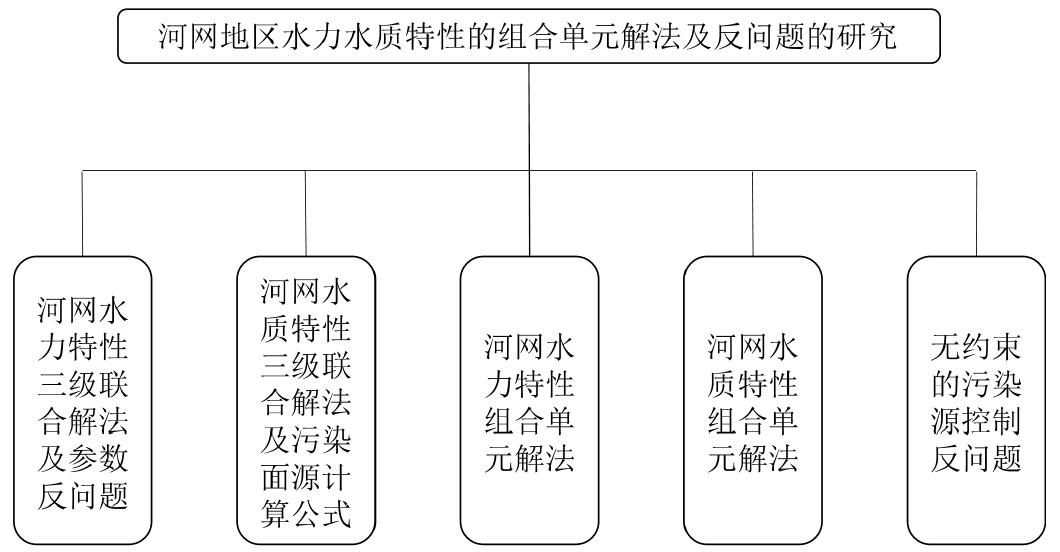
\includegraphics[width=0.75\textwidth]{figure1.jpg}
	\caption{论文的主要研究内容} 
	\label{fig:maincontents}
	%硕士论文、本科毕业论文不使用双语图表标题,可使用命令\caption{}替代\caption{}
\end{figure}

